
%(BEGIN_QUESTION)
% Copyright 2008, Tony R. Kuphaldt, released under the Creative Commons Attribution License (v 1.0)
% This means you may do almost anything with this work of mine, so long as you give me proper credit

The {\it HART} protocol was an early attempt at establishing a digital communications standard for field process instruments, designed as an extension of the already-popular 4 to 20 mA DC current signal standard.  The basic idea of HART is that serial digital data could be encoded as bursts of high-frequency AC voltage superimposed on the DC voltage present in a 4-20 mA loop-powered circuit:

$$\includegraphics[width=15.5cm]{i00400x01.eps}$$

A microprocessor inside the loop-powered transmitter detects the digital data signals from the HART communicator as pulses of low-voltage AC dropped across the transmitter terminals.  The transmitter, in turn, has the ability to send digital data out in the same format, being detected by the communicator as AC voltage pulses across its terminals.

Apply the Superposition Theorem to this circuit, showing the circuit as ``seen'' by the AC signals sent between the transmitter and communicator, and showing the circuit as ``seen'' by the DC signals sent between the transmitter and the indicator.

\vskip 10pt

Also, identify where in the circuit the communicator may be connected and still be able to ``talk'' with the smart instrument.  What advantage(s) may there be in being able to connect the communicator at different points in the circuit?

\underbar{file i00400}
%(END_QUESTION)





%(BEGIN_ANSWER)

\noindent
{\bf Circuit as it appears to AC (HART) signals sent by the communicator:}

$$\includegraphics[width=15.5cm]{i00400x02.eps}$$

\vskip 10pt

\noindent
{\bf Circuit as it appears to DC (4-20 mA) signals:}

$$\includegraphics[width=15.5cm]{i00400x03.eps}$$

\vskip 10pt

The communicator may be connected {\it anywhere} that places it in parallel with the transmitter terminals, from the transmitter itself all the way back to the control panel where the indicator is located!

\vskip 10pt

Challenge question: a HART communicator will be able to communicate with the smart field instrument if it is connected directly in parallel with the 250 $\Omega$ loop resistor, even though this is technically not in parallel with the transmitter terminals.  Explain why this works!

%(END_ANSWER)





%(BEGIN_NOTES)

Note that the transmitter is not a true source of power as its current-source symbol suggests.  Rather, it functions as a current {\it regulator}.  The actual power source is the 24 volt DC battery.  However, it is still valid to eliminate the 24 volt DC battery for the purpose of analysis with Superposition, just to show the signal paths.

Also note that the HART signal gets impressed across the 250 ohm resistor just as much as it gets sent to the transmitter.  This means the HART communicator has the ability to interfere with the process signal received by the indicator or controller!  In most cases, the low-pass input filtering of these devices prevents any problem, but this is not always the case.  I have personally seen controllers exhibit fluctuations in their process variable displays when a HART communicator was ``talking'' on the loop.  For this reason (and for others), it is not a bad idea to set the controller into {\it manual} mode when digitally communicating with the transmitter.

\vskip 10pt

It is important to discuss with your students the possibility of connecting a HART communicator {\it anywhere} on the loop circuit placing it parallel with the transmitter terminals.  This freedom allows technicians to check parameters and perform re-ranging on a field-mounted transmitter from the convenience of the control room.  It also means HART-compatible control systems (such as many modern distributed control systems, or DCS's) have the ability to do access smart instrument parameters without the necessity of additional connections to the instrument other than the existing 4-20 mA pair cable.

A parallel connection across the 250 $\Omega$ resistor is possible because the DC voltage source is ``seen'' by HART signals from both the communicator and the transmitter as a short-circuit.

%INDEX% Fieldbus, HART: analysis of 4-20 mA / HART transmitter circuit using Superposition Theorem

%(END_NOTES)


